\begin{figure}
	\centering
	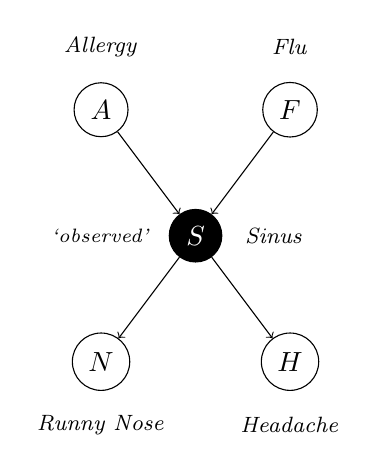
\begin{tikzpicture}[
		scale=0.8
	]

		\node[circle,draw=black] (A) at (-1.5,2) {$A$}; \node at (-1.5,3) {\footnotesize \textit{Allergy}};
		\node[circle,draw=black] (F) at (1.5,2) {$F$}; \node at (1.5,3) {\footnotesize \textit{Flu}};
		\node[circle,draw=black,fill=black,text=white] (S) at (0,0) {$S$}; \node at (1.25,0) {\footnotesize \textit{Sinus}};
			\node at (-1.5,0) {\scriptsize \textit{`observed'}};
		\node[circle,draw=black] (N) at (-1.5,-2) {$N$}; \node at (-1.5,-3) {\footnotesize \textit{Runny Nose}};
		\node[circle,draw=black] (H) at (1.5,-2) {$H$}; \node at (1.5,-3) {\footnotesize \textit{Headache}};

		\draw[->] (A) -- (S);
		\draw[->] (F) -- (S);
		\draw[->] (S) -- (N);
		\draw[->] (S) -- (H);

	\end{tikzpicture}
\end{figure}